\chapter{Анализ спектральных данных}
\label{cha:ch_5}

В качестве исследования были обработаны сырые спектральные данные, полученные при одних и тех же
технических условиях системы, в отсутствие пылевого облака, а также в присутствии пылевого облака (см~рис.~\ref{fig:fig34}).

\begin{figure}[t]
    \centering
    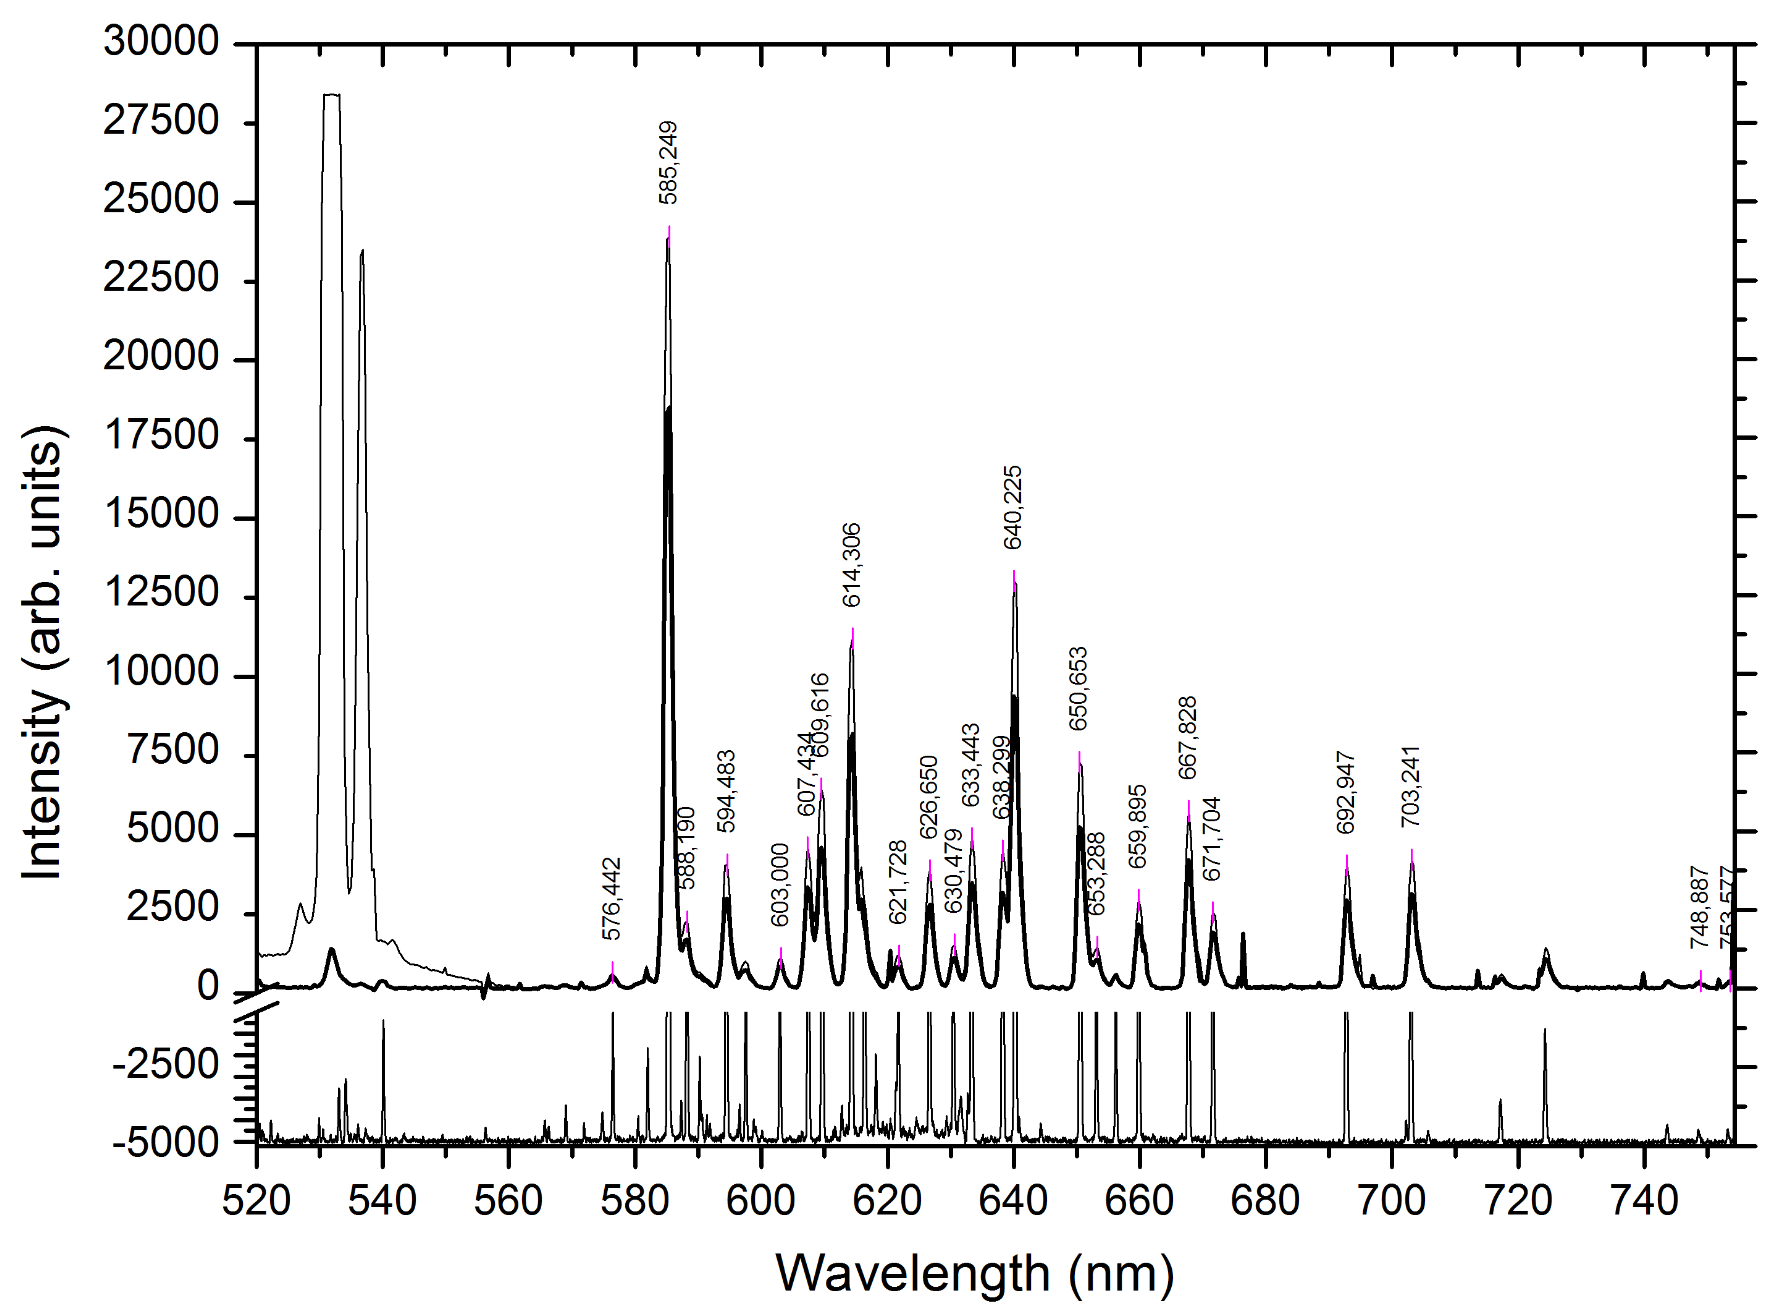
\includegraphics[width=16cm]{figures/fig34}
    \caption{
        Зависимость интенсивности (усл.~ед.) от длины волны (нм). На графике наложены три спектра:
        1. Ниже нуля калибровочный спектр с достоверными линиями неона;
        2. Жирной линией выделен спектр без пылевого облака.
        3. Тонкой линией выделен спектр с пылевым облаком
    }
    \label{fig:fig34}
\end{figure}


Экспериментально было обнаружено увеличение интенсивности спектральных линий при попадании пылевого облака
в газовый разряд неона, причем линии с разными верхними энергетическими уровнями имеют разные значения
отношений интенсивностей (см~рис.~\ref{fig:fig35}).
\begin{figure}[t]
    \centering
    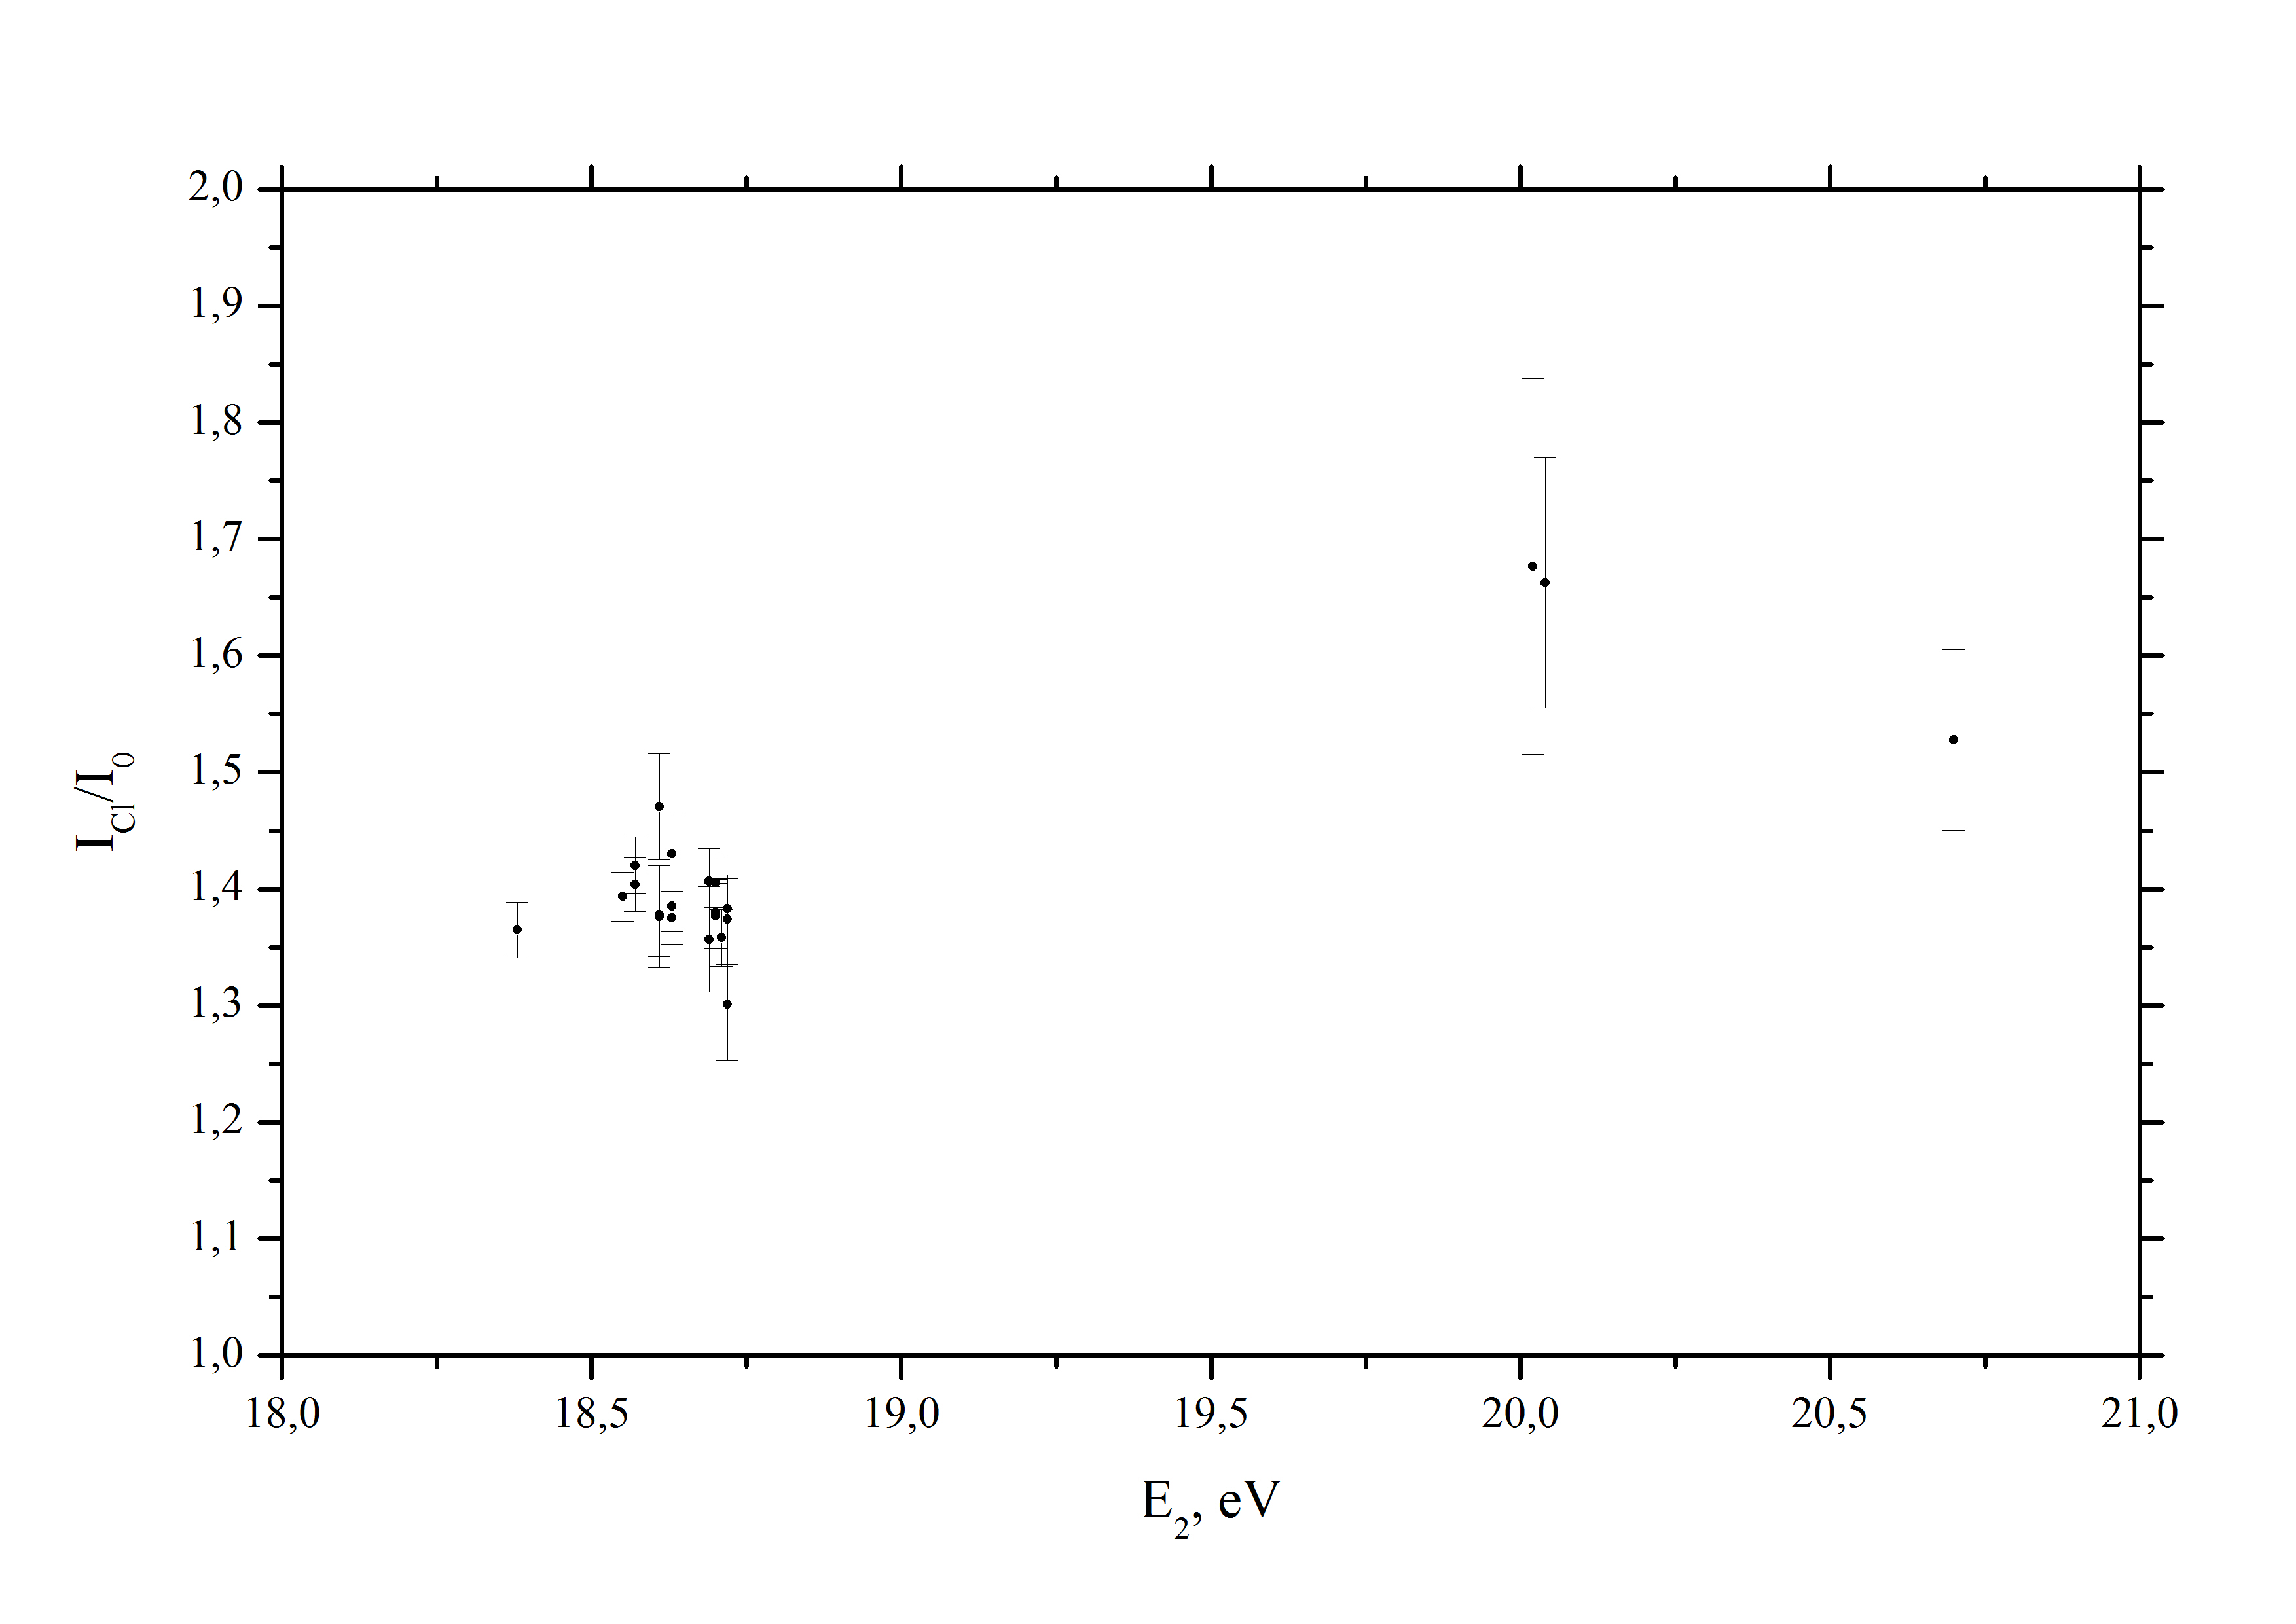
\includegraphics[width=16cm]{figures/fig35}
    \caption{Зависимость отношения интенсивностей спектральных линий неона в присутствии пылевого облака к отсутствию пылевого облака.}
    \label{fig:fig35}
\end{figure}


% [МОЖЕТ СТОИТ ВЫНЕСТИ ДАЛЬНЕЙШИЕ РАССУЖДЕНИЯ В РАЗДЕЛ "АНАЛИЗ СПЕКТРАЛЬНЫХ ДАННЫХ" ???]





% ПЕРЕНЕСТИ
\begin{figure}[t]
  \centering
  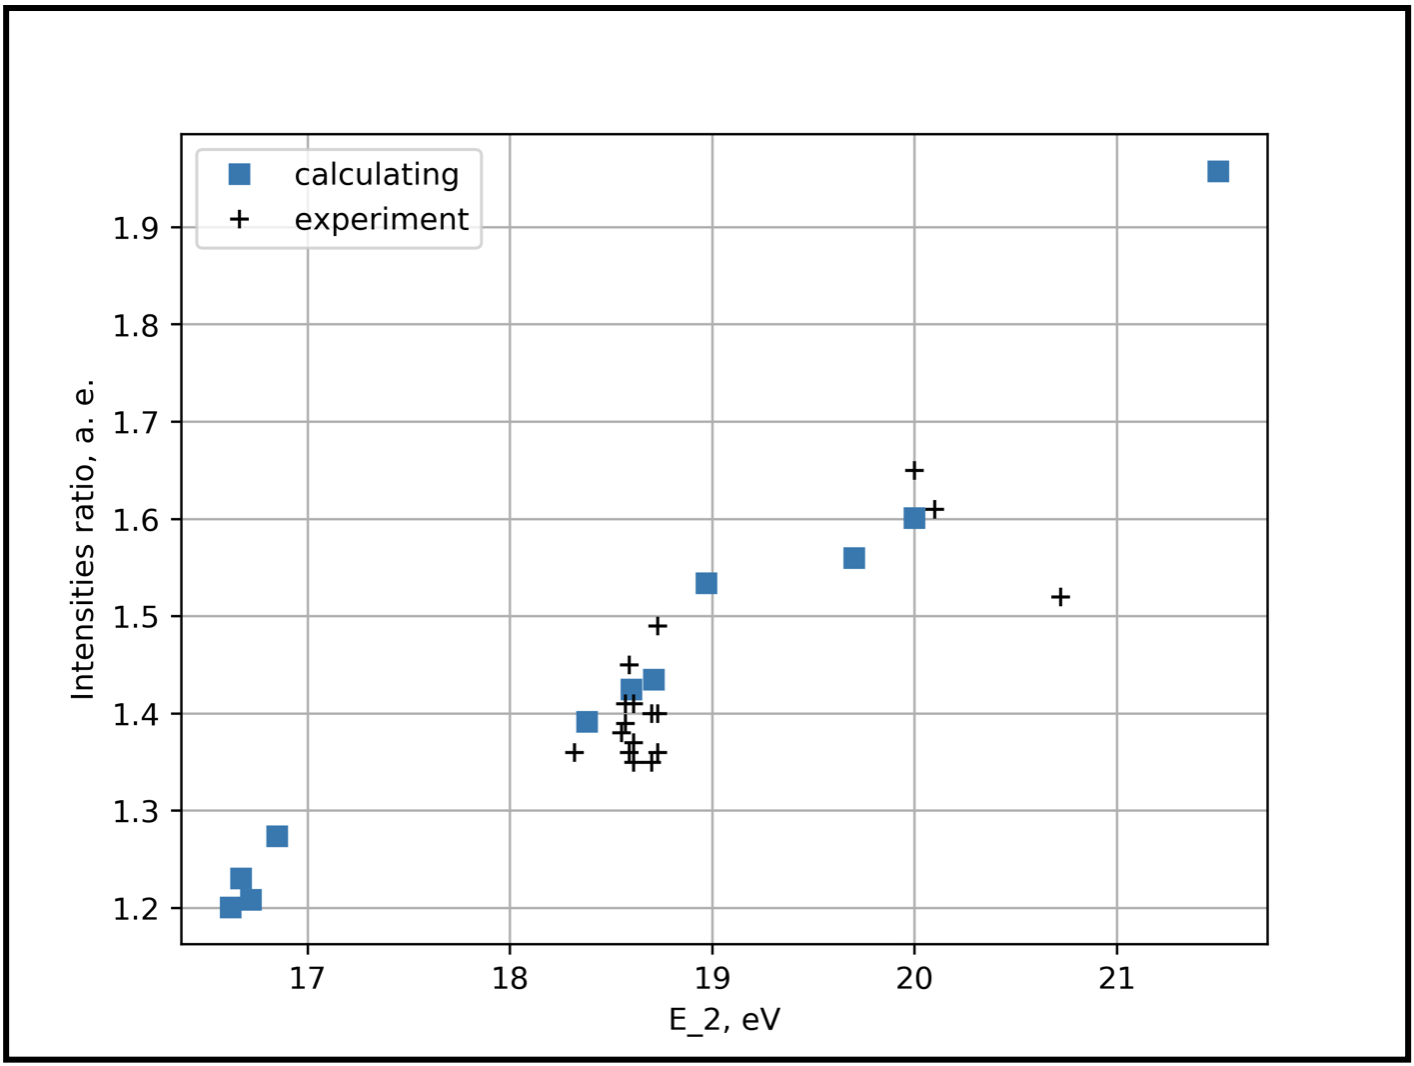
\includegraphics[width=16cm]{figures/fig16}
  \caption{Зависимость ...... .}
  \label{fig:fig16}
\end{figure}
